\chapter{Объект 5. Что ты такое}

Рассмотрим схему регулятора на операционном усилителе:

\begin{figure}[H]
    \centering
    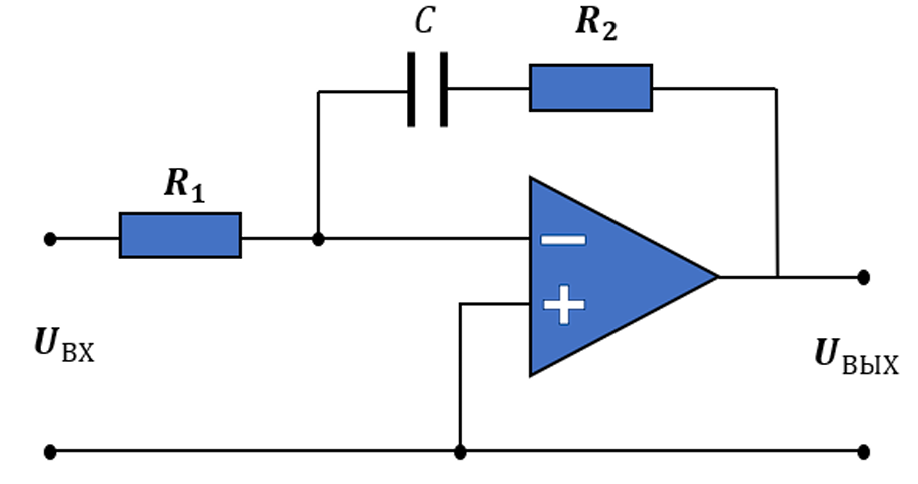
\includegraphics[width=0.75\textwidth, trim={0cm 0cm 0cm 0cm}]{../images/scheme.png}
    \caption{Схема регулятора на операционном усилителе}
\end{figure}

со следующими параметрами:
\begin{itemize}
    \item[] \( R_1 = 2425\, \text{Ом} \)
    \item[] \( R_2 = 21827\, \text{Ом} \)
    \item[] \( C = 324\, \text{мкФ} \)
\end{itemize}

Присмотревщись к схеме, можно заметить, что она 
представляет собой пропорционально-интегрирующее звено, которое
имеет передаточную функцию вида:
\[
    W(s) = \frac{K(Ts + 1)}{Ts}
\]

Для представленного регулятора коэффициенты \( K \) и \( T \) равны:
\[
    K = \frac{R_2}{R_1} = 9.008, \quad T = R_2 C = 7.0719
\]

\section{Временные характеристики}

Переходная характеристика для пропорционально-интегрирующего звена имеет вид:
\[
    h(t) = K \left( 1 + {t}{T} \right)
\]

Весовая характеристика для пропорционально-интегрирующего звена имеет вид:
\[
    w(t) = \frac{K}{T}
\]

\begin{figure}[H]
    \centering
    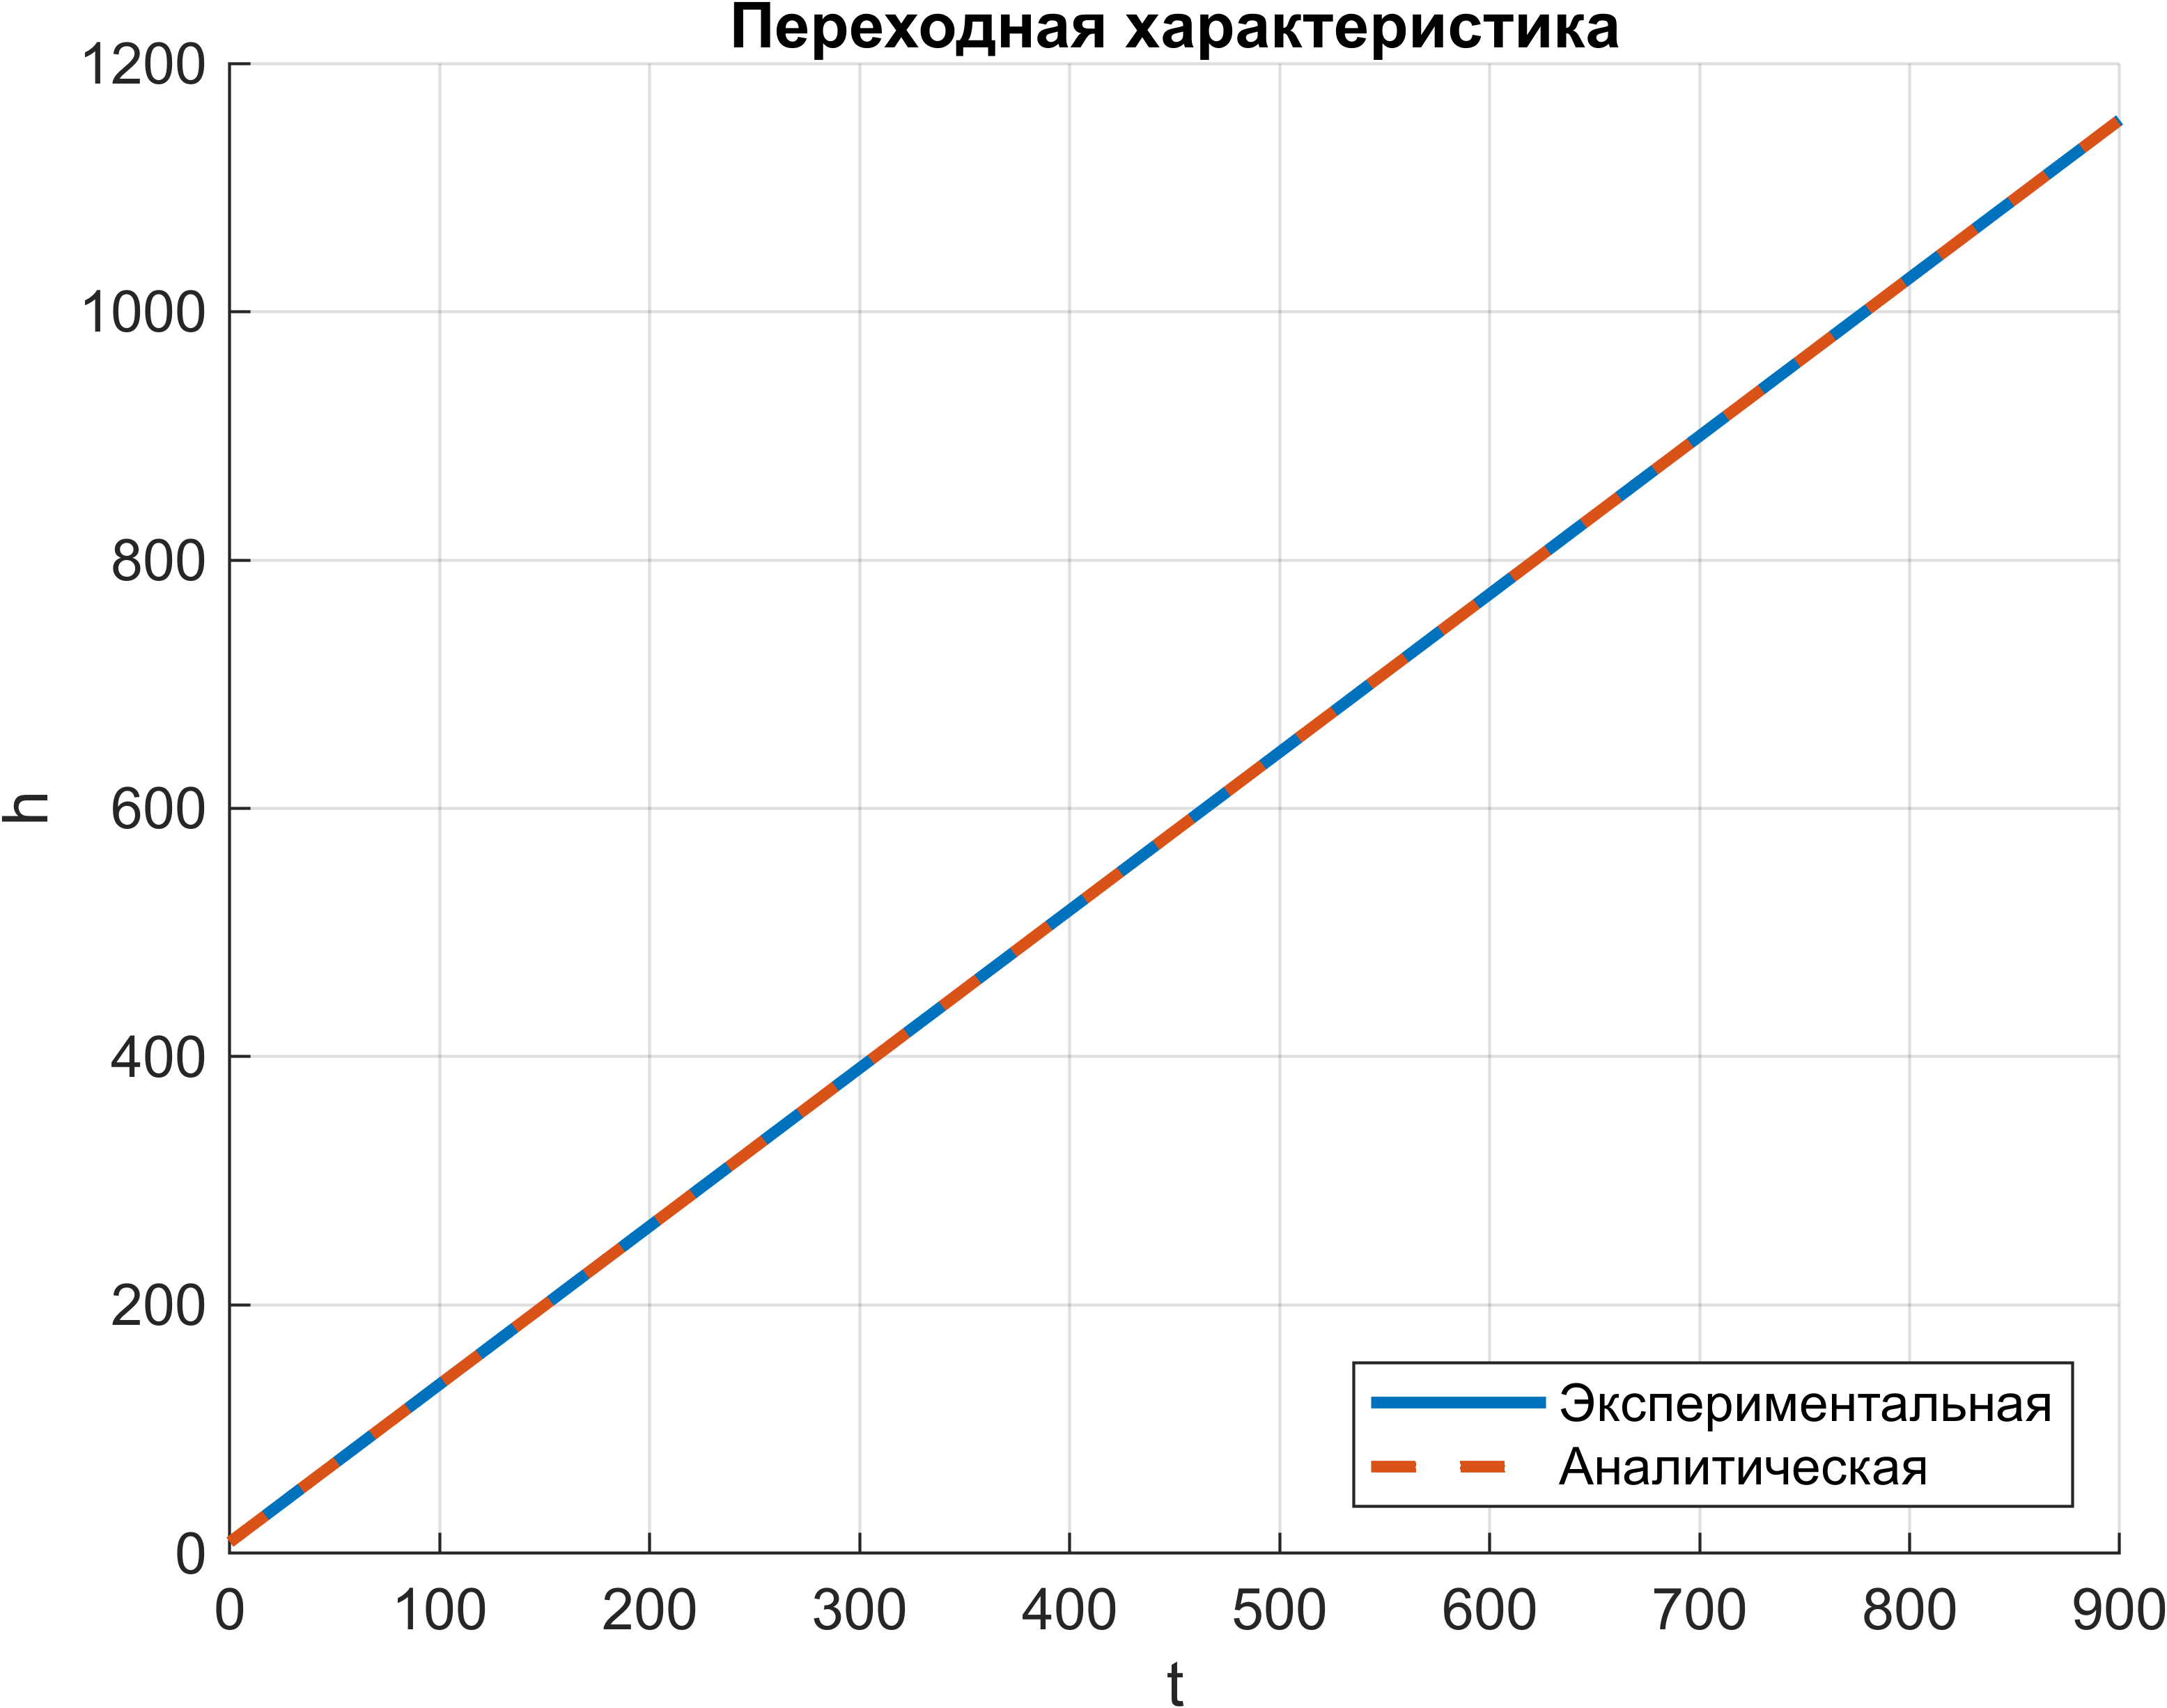
\includegraphics[width=0.75\textwidth, trim={0cm 0cm 0cm 0cm}]{../images/5_1.png}
    \caption{Переходная характеристика регулятора}
\end{figure}

\begin{figure}[H]
    \centering
    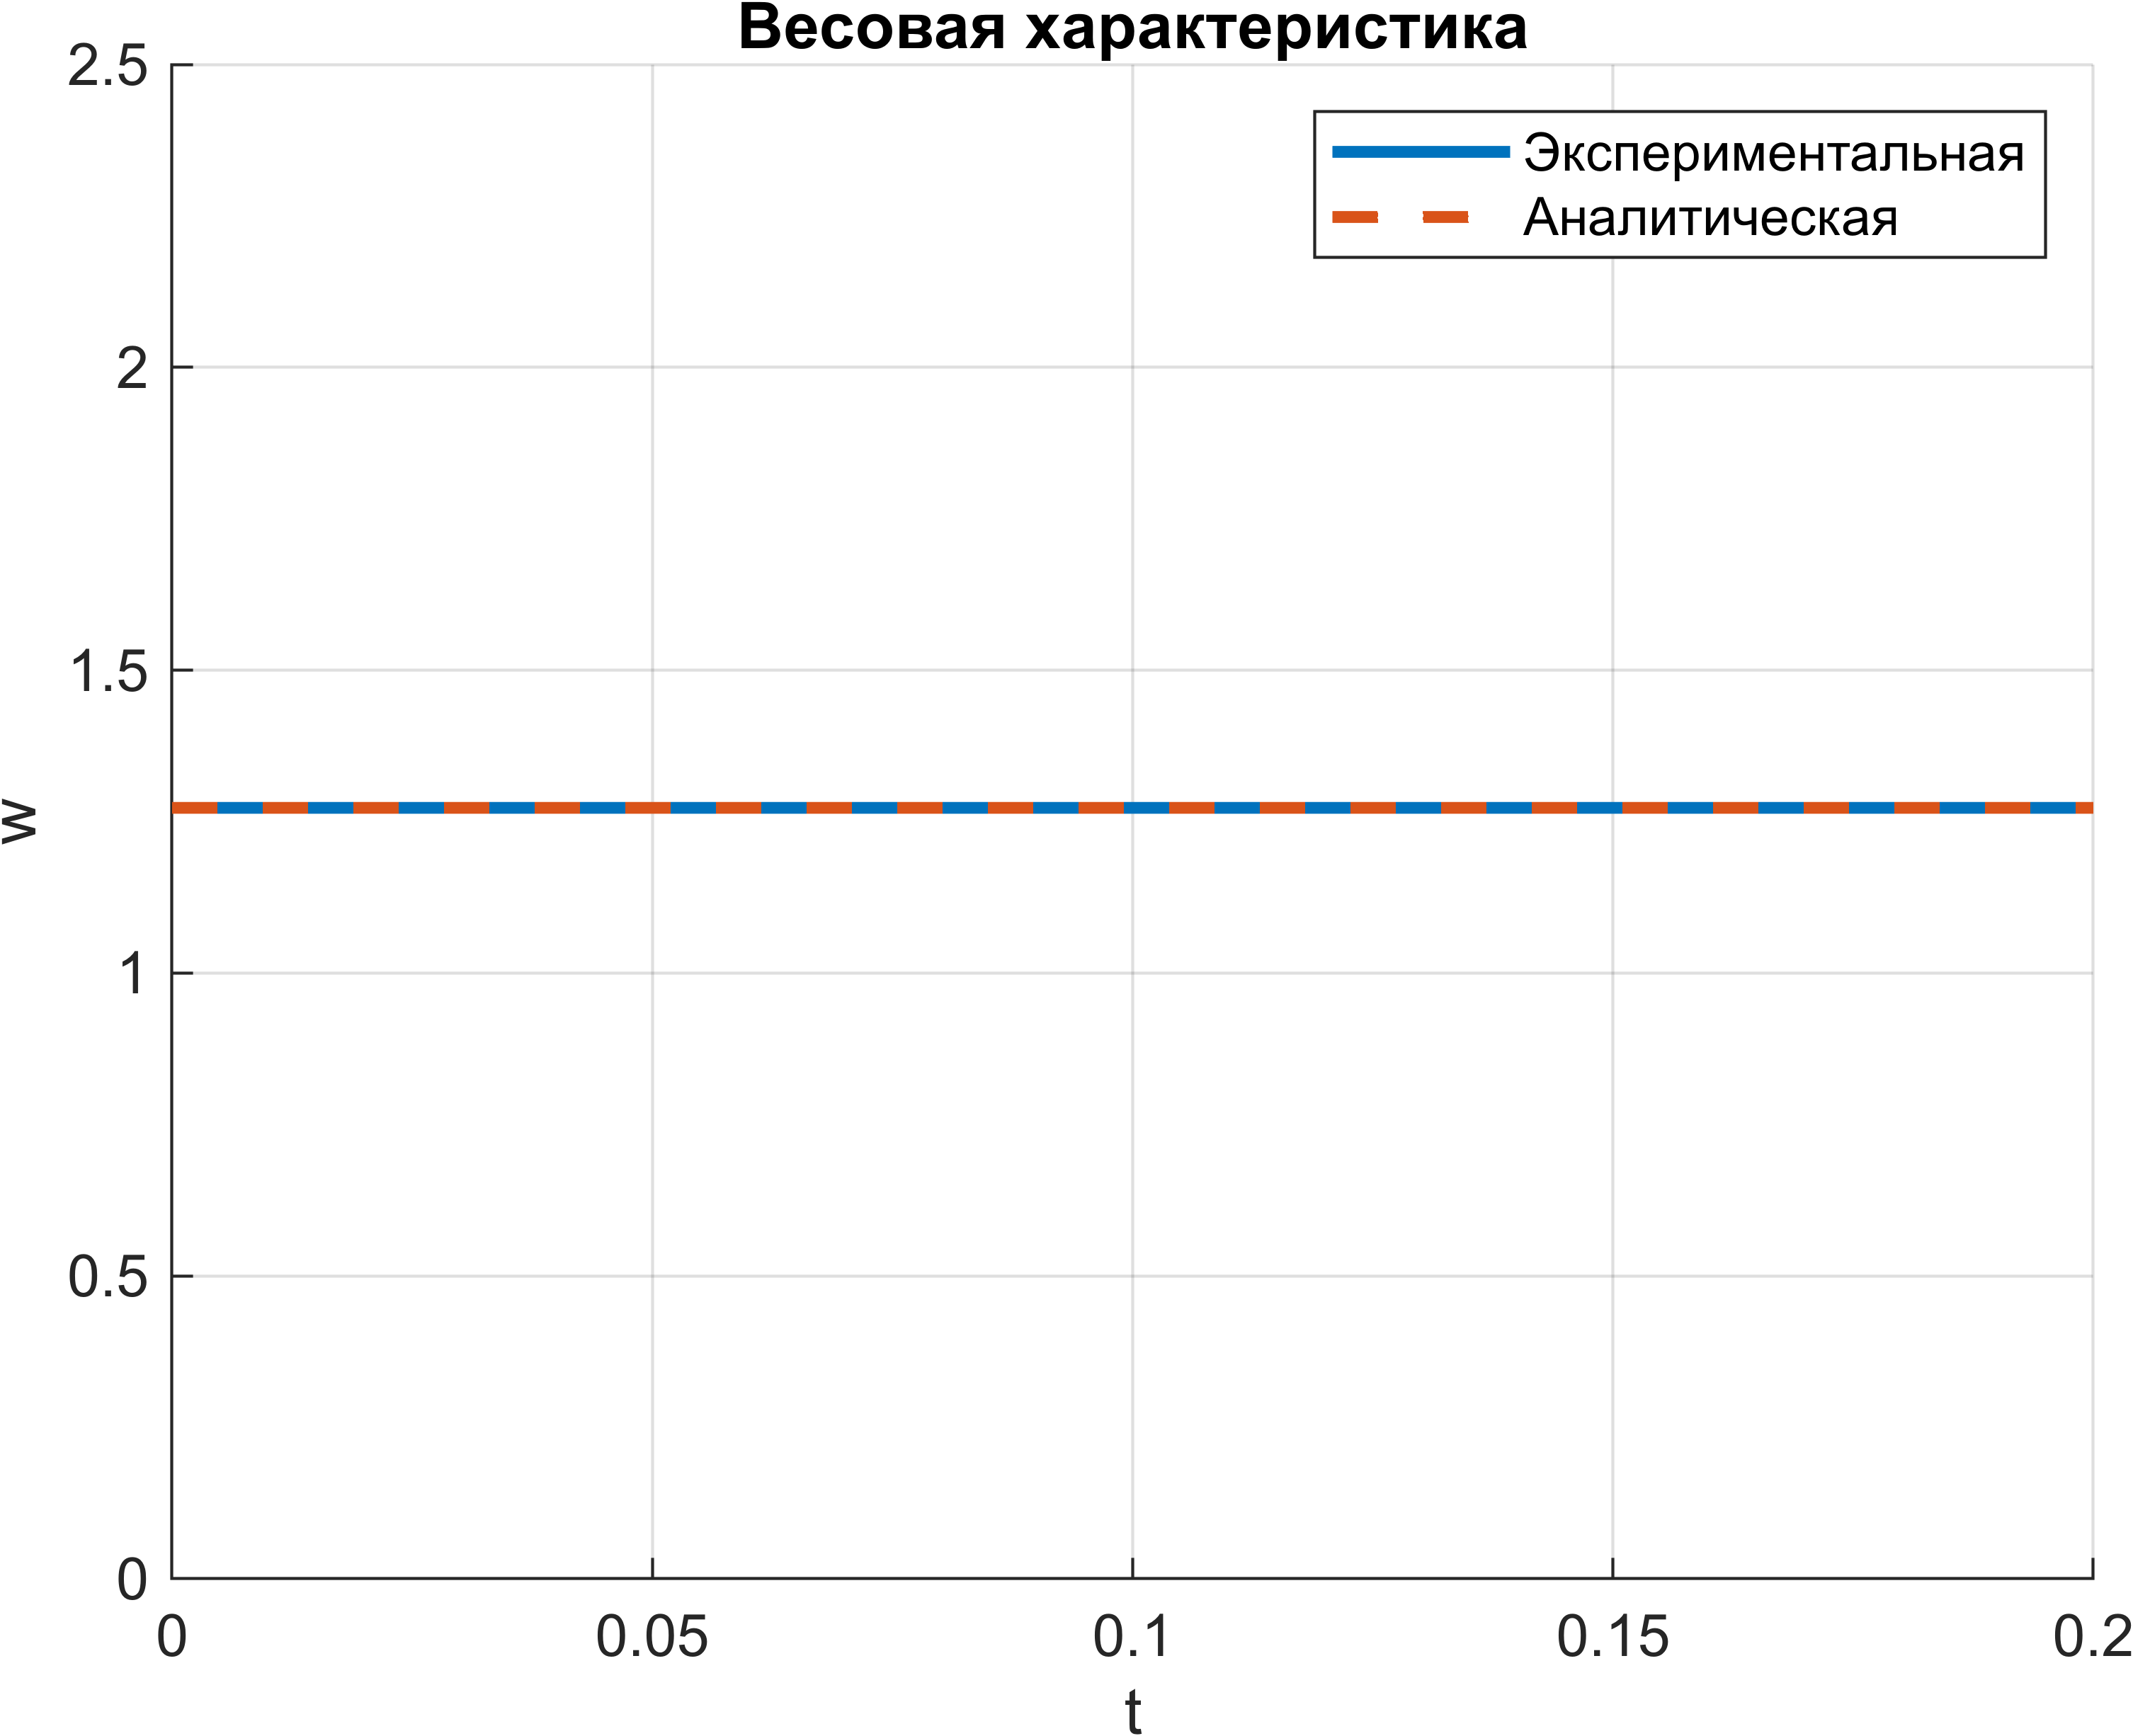
\includegraphics[width=0.75\textwidth, trim={0cm 0cm 0cm 0cm}]{../images/5_2.png}
    \caption{Весовая характеристика регулятора}
\end{figure}

\section{Частотные характеристики}

Амплитудно-частотная характеристика для пропорционально-интегрирующего звена имеет вид:
\[
    A(\omega) = \frac{K\sqrt{1 + \omega^2 T^2}}{\omega T}
\]

Логарифмическая амплитудно-частотная характеристика:
\[
    \lg A(\omega) = 20\lg K + 10\lg(1 + \omega^2 T^2) - 20\lg\left(\omega T\right)
\]

Фазо-частотная характеристика для пропорционально-интегрирующего звена имеет вид:
\[
    \varphi(\omega) = -\arctan\left(\frac{1}{\omega T}\right)
\]

\begin{figure}[H]
    \centering
    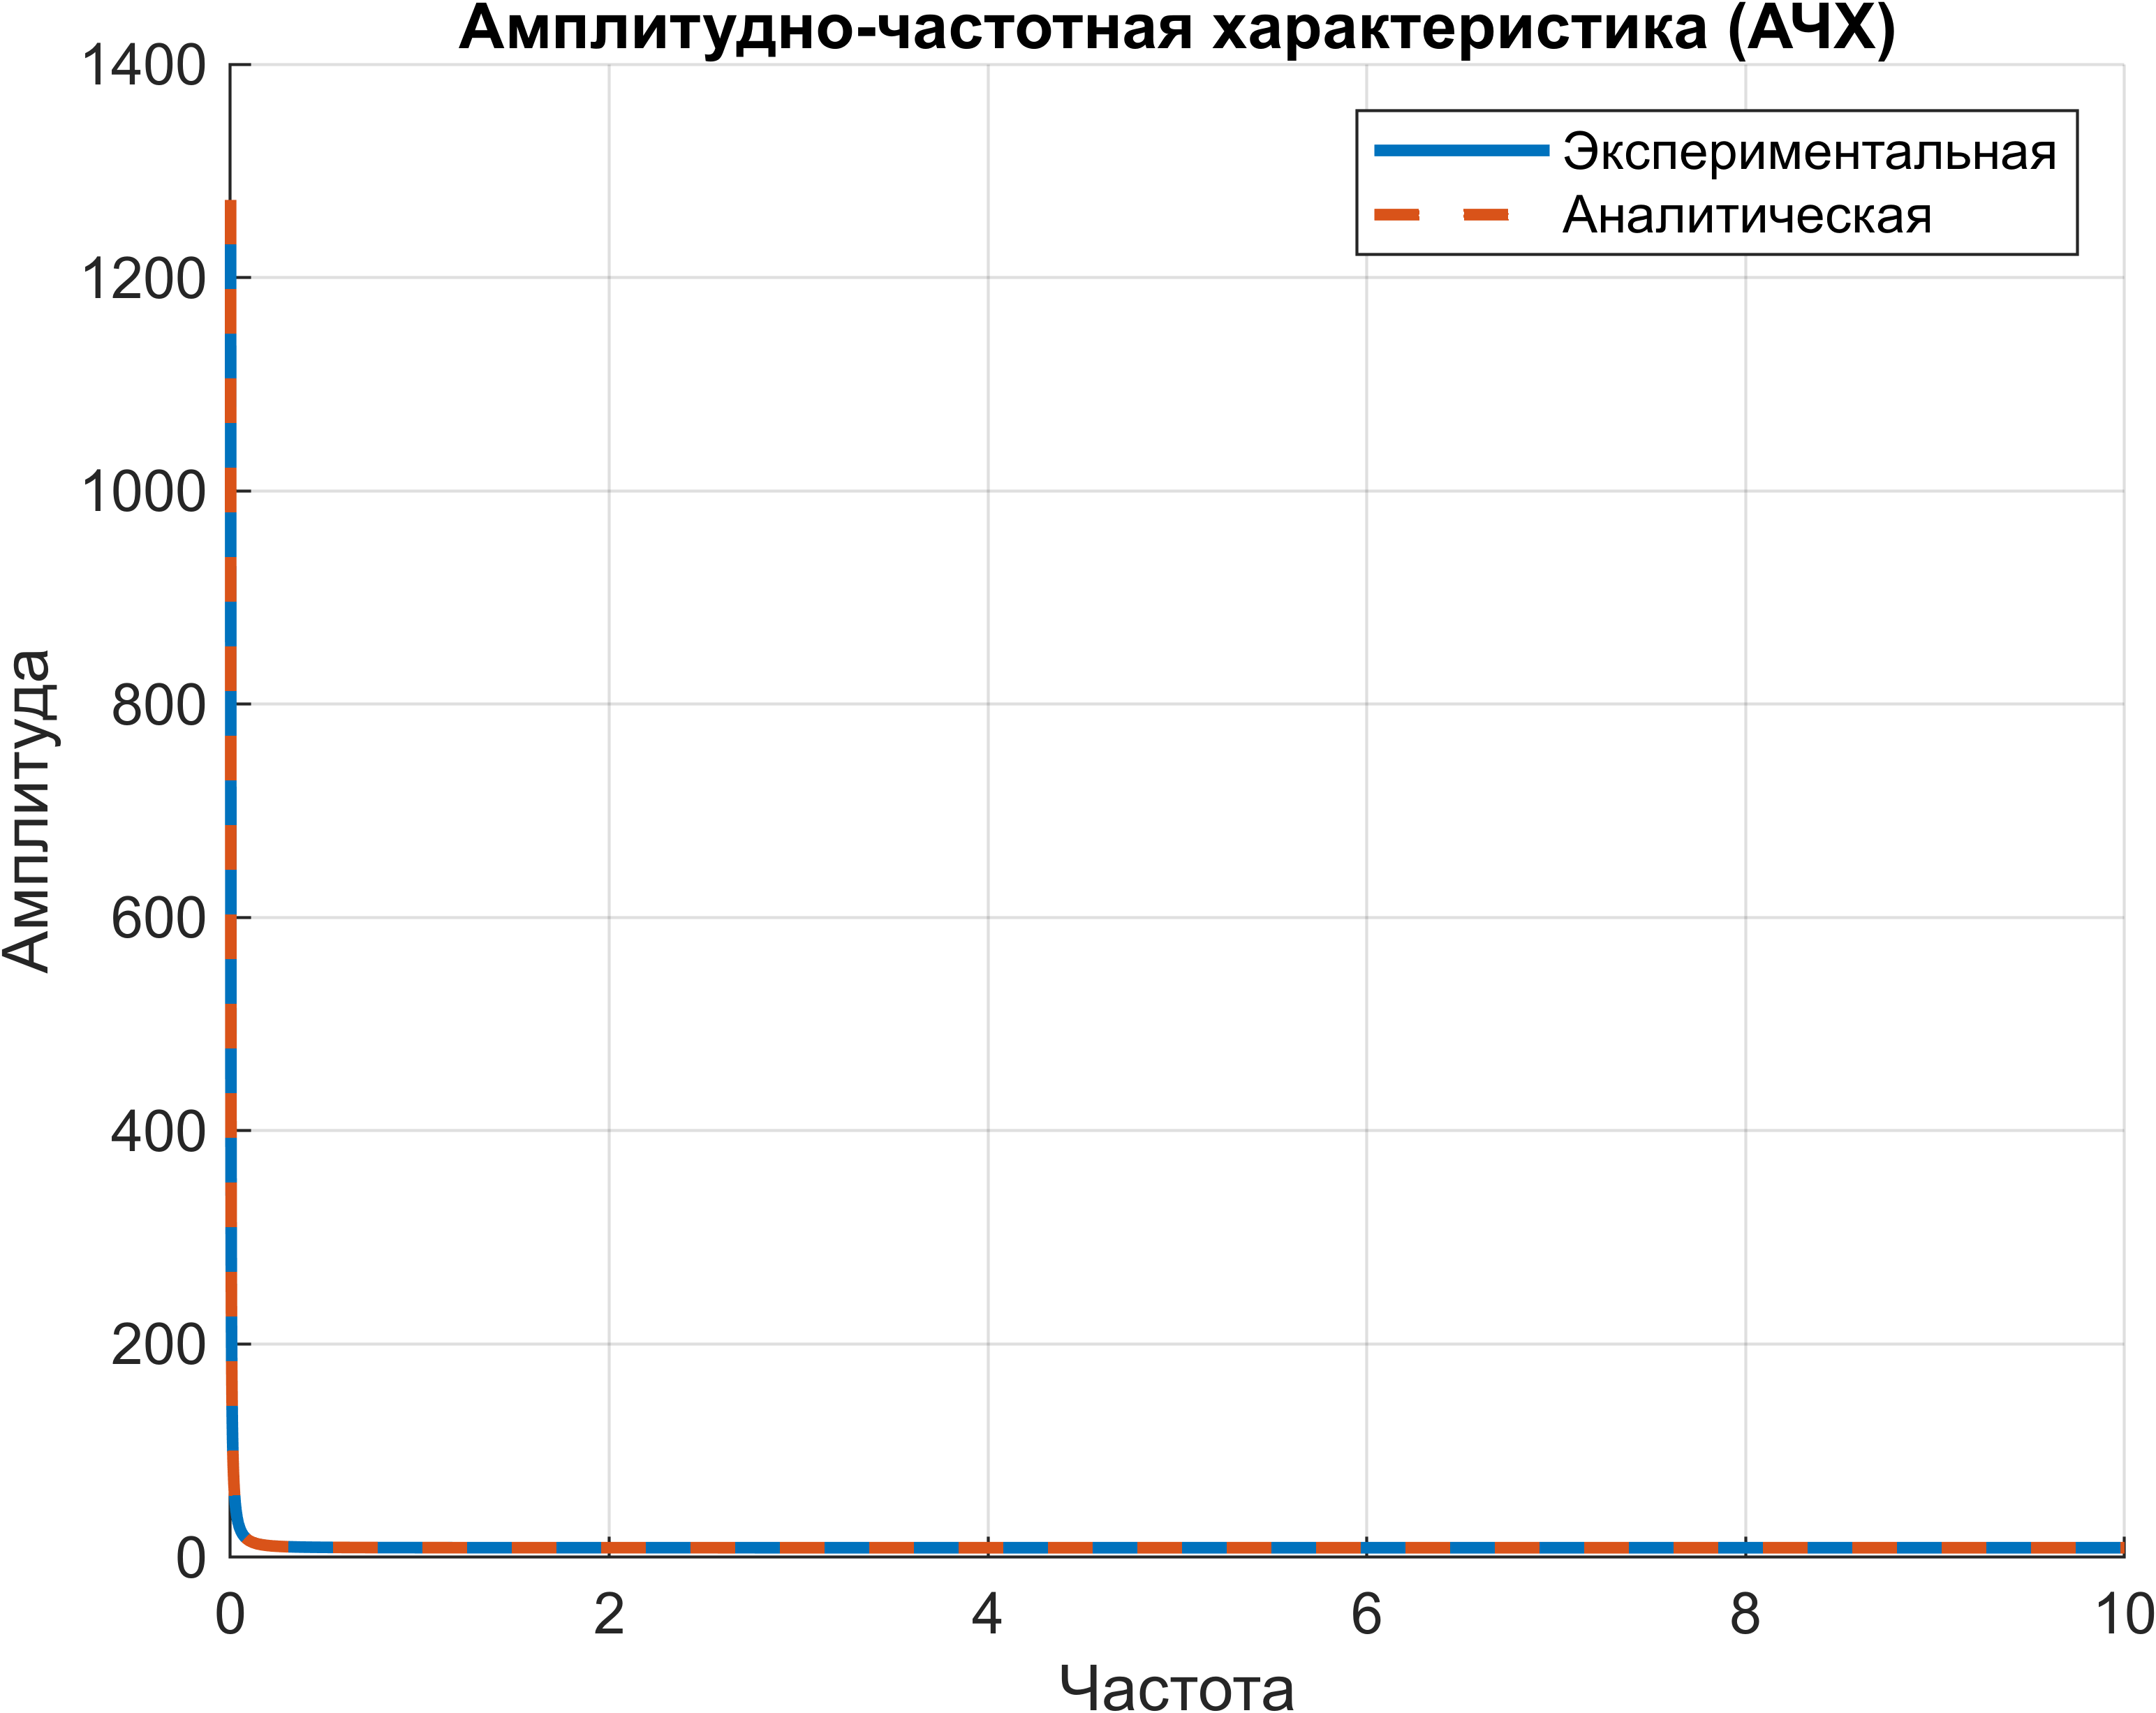
\includegraphics[width=0.75\textwidth, trim={0cm 0cm 0cm 0cm}]{../images/5_3.png}
    \caption{Амплитудно-частотная характеристика регулятора}
\end{figure}

\begin{figure}[H]
    \centering
    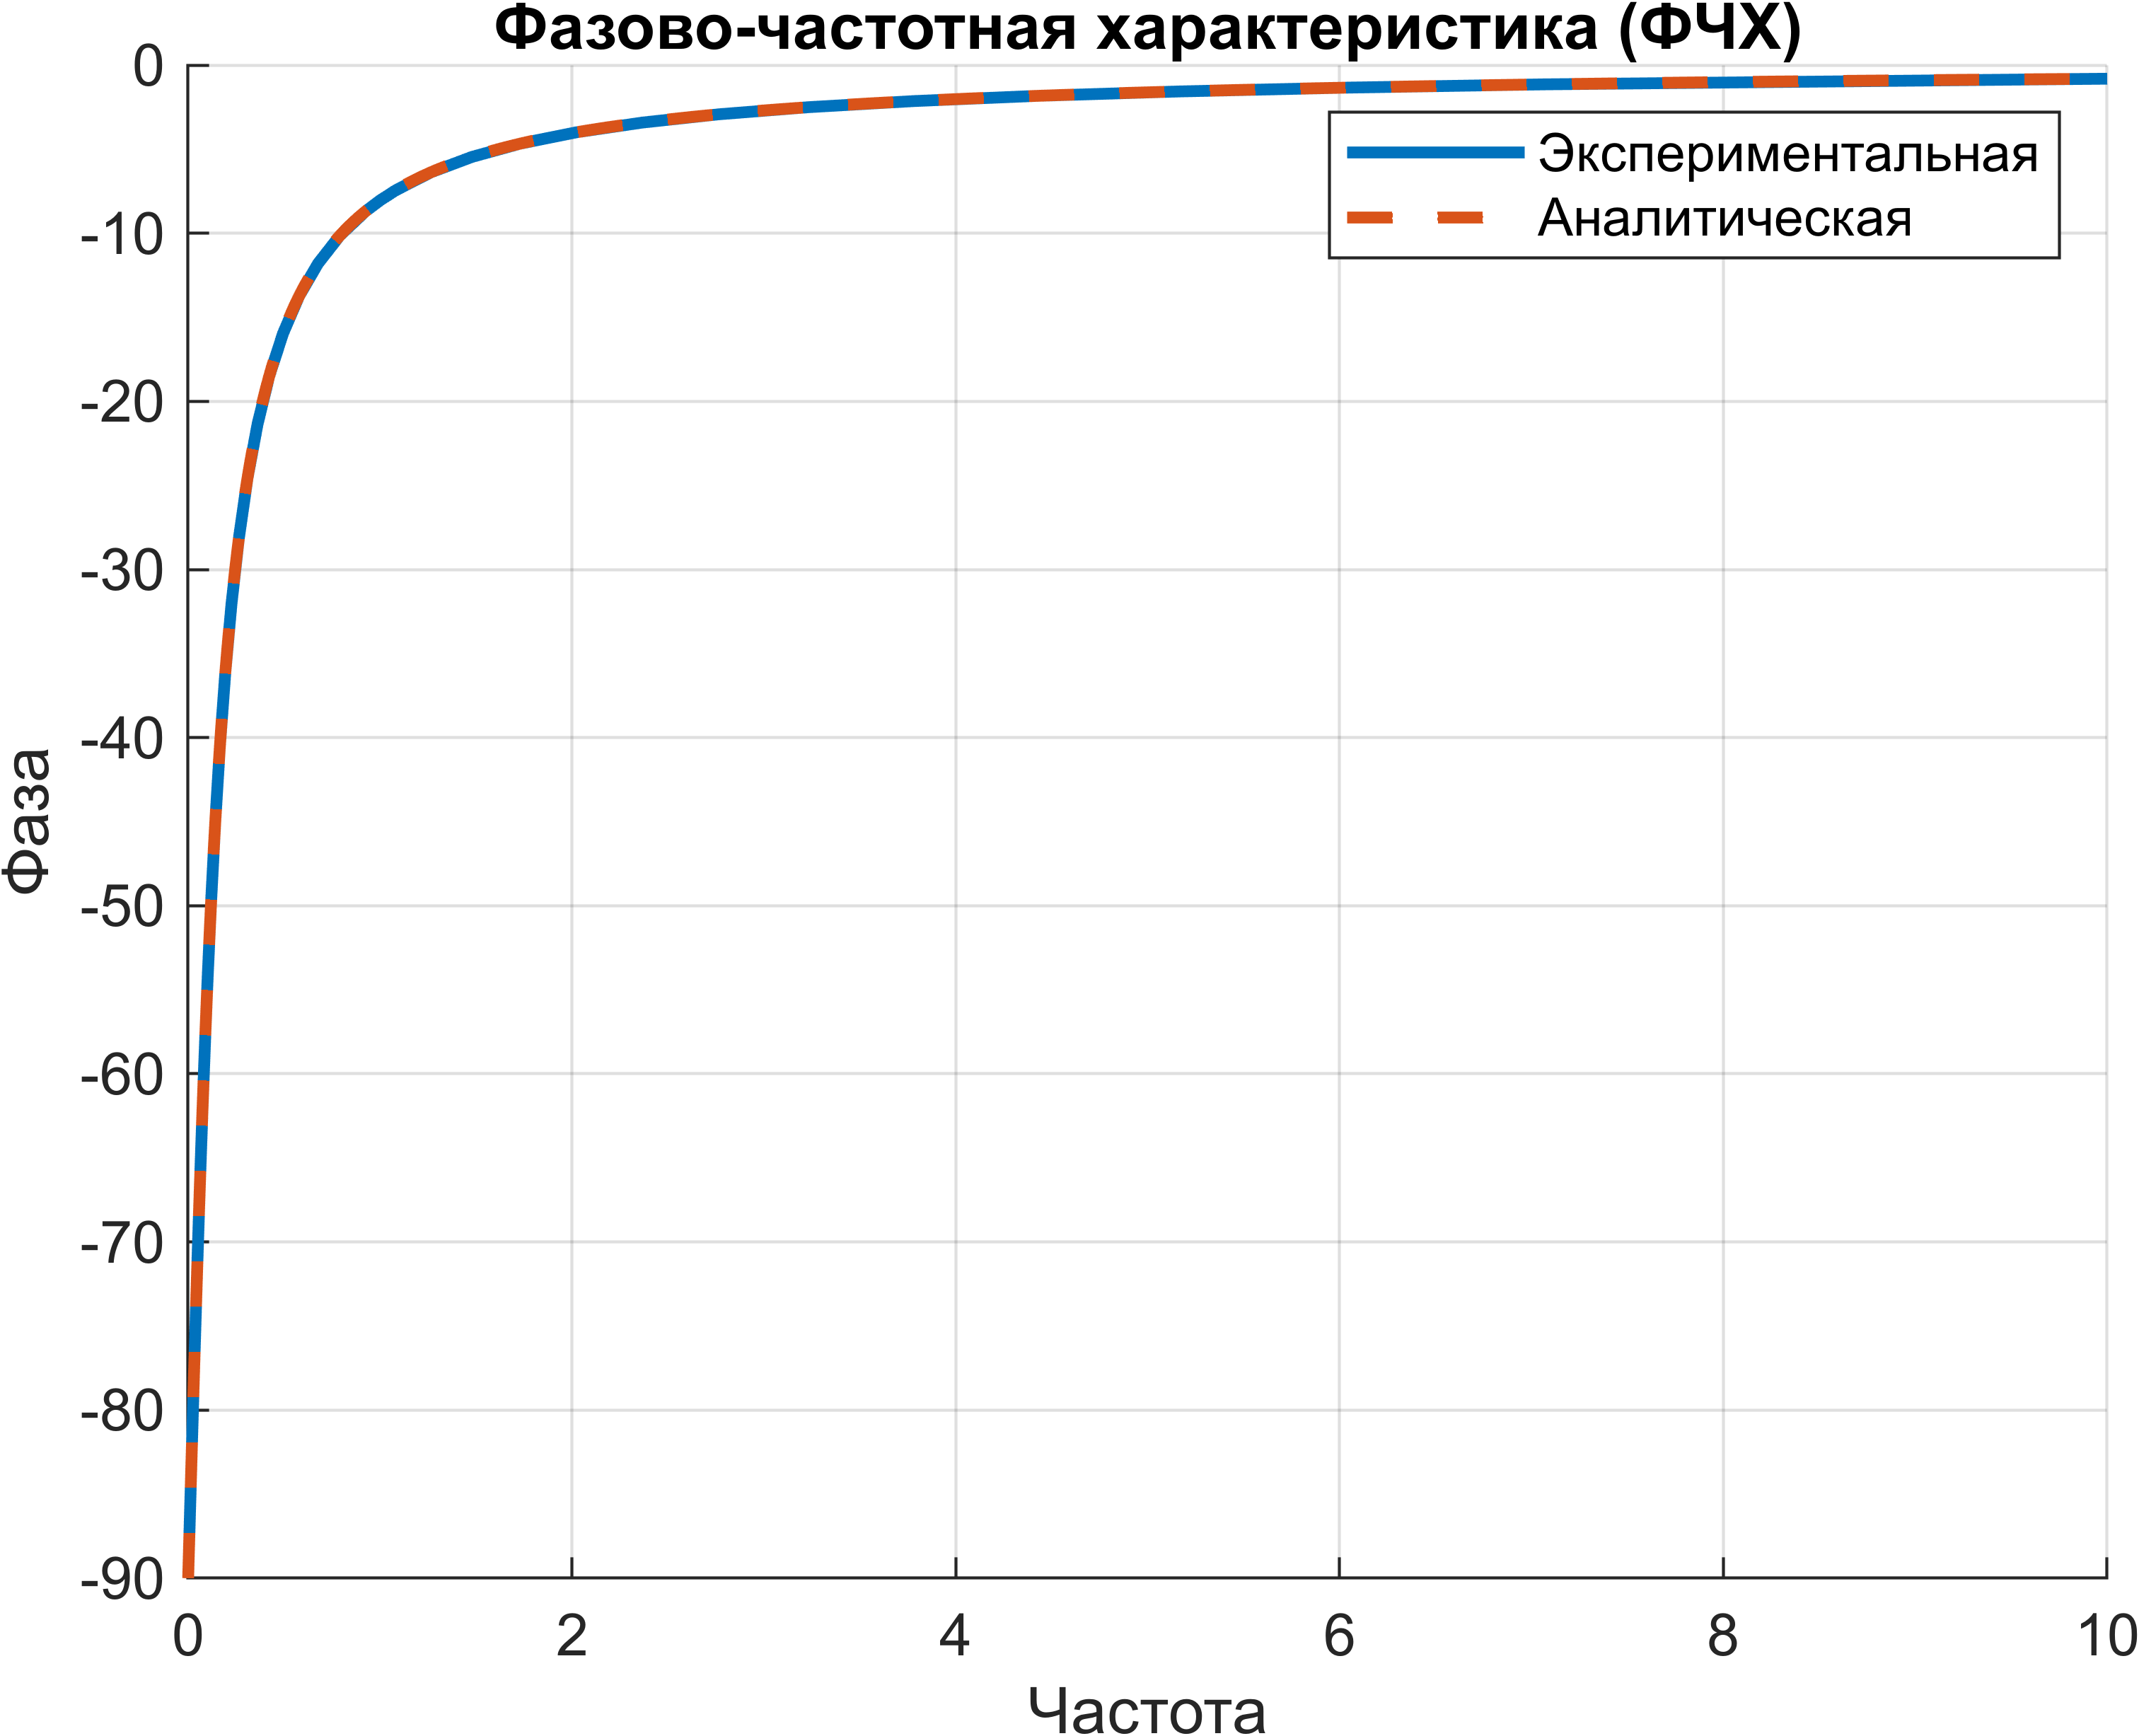
\includegraphics[width=0.75\textwidth, trim={0cm 0cm 0cm 0cm}]{../images/5_4.png}
    \caption{Фазо-частотная характеристика регулятора}
\end{figure}

\begin{figure}[H]
    \centering
    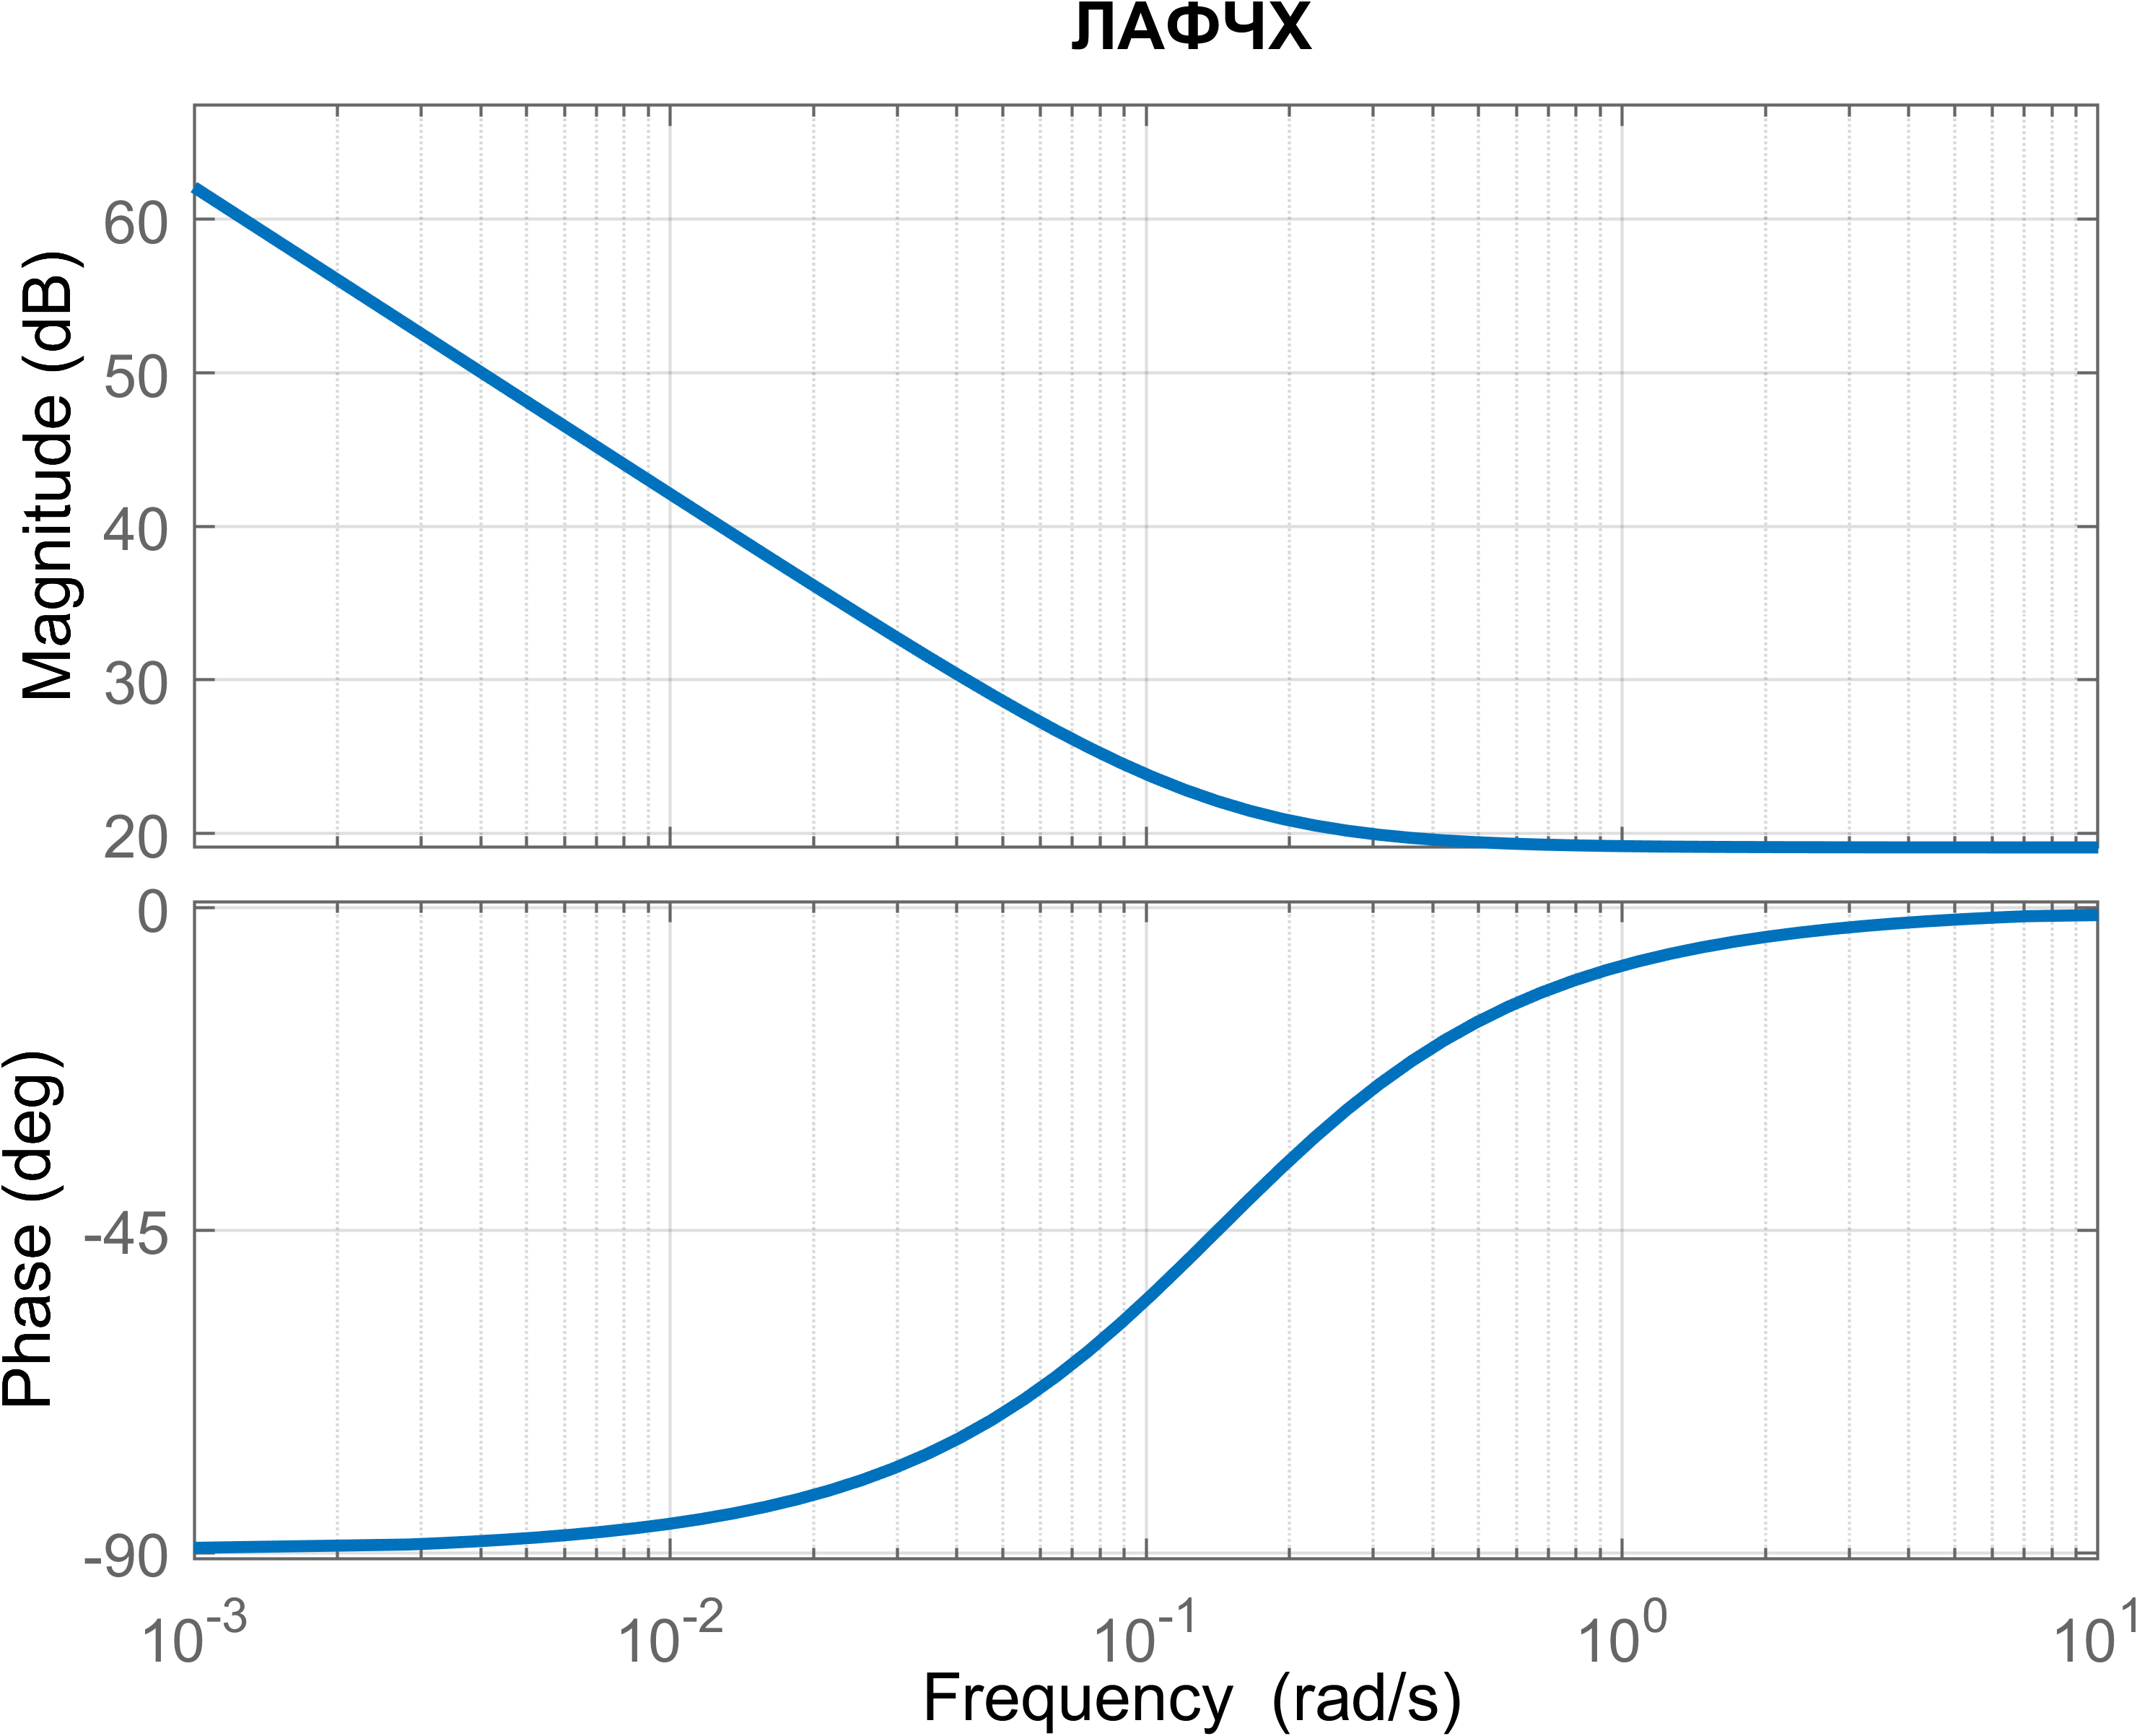
\includegraphics[width=0.75\textwidth, trim={0cm 0cm 0cm 0cm}]{../images/5_5.png}
    \caption{Логарифмическая амплитудно-фазо-частотная характеристика регулятора}
\end{figure}
\endinput